%\documentclass[1p,12pt]{elsarticle}
\documentclass[aps,prl,twocolumn,showpacs,superscriptaddress,groupedaddress]{revtex4}  % for review and submission

\usepackage{graphicx}
\usepackage{dcolumn}
\usepackage{bm}        % for math
\usepackage{amssymb}   % for math
\usepackage{mathtools}
\usepackage{verbatim}

\newcommand{\Phperp}{P_{h\perp}}
\newcommand{\FUUc}{F_{UU}^{\cos\phi}}
\newcommand{\FUUcc}{F_{UU}^{\cos2\phi}}
\newcommand{\kt}{\vec{k}_\perp}
\newcommand{\pt}{\vec{p}_\perp}
\newcommand{\zh}{z}
\newcommand{\xbj}{x}
\newcommand{\PT}{P_T}                   % Bjorken variable
\newcommand{\ph}{\phi_h}
\newcommand{\la}{\langle}
\newcommand{\ra}{\rangle}

\begin{document}
\widetext
\newcommand*{\JLAB}{Thomas Jefferson National Accelerator Facility, Newport News, Virginia 23606}
\affiliation{\JLAB}

\title{Exploring the Structure of the Proton via Semi-inclusive Pion Electroproduction}


\author{N.~Harrison et al}
\affiliation{\JLAB}
\collaboration{The CLAS Collaboration}
     \noaffiliation

%%%%%%
\date{\today}
\begin{abstract}


We present studies of the $\cos\phi_h$ and $\cos2\phi_h$ moments and the $\phi_h$-independent term of the semi-inclusive deep inelastic scattering (SIDIS) cross-section in charged pion production.
The data set used was the E1-f run from the CEBAF Large Acceptance Spectrometer (CLAS) at Jefferson Lab which ran in 2003.
The run used a 5.498 GeV longitudinally polarized electron beam and an unpolarized liquid hydrogen target.
Two pion channels ($\pi^+$ and $\pi^-$) were studied over a broad kinematical range ($x = 0.1 - 0.6$, $Q^2 = 1.0 - 4.5\ \text{GeV}^2$, $z = 0.0 - 0.9$, $P_{h\perp}^2 = 0.0 - 1.0\ \text{GeV}^2$, and $-180^\circ < \phi_h < 180^\circ$).
These measurements give insights into the transverse momentum dependence of parton distribution functions (PDFs) describing the dynamics of quarks and gluons inside of the proton.

\end{abstract}

%\pacs{13.60.-r \sep 13.87.Fh \sep 13.88.+e \sep 14.20.Dh \sep 24.85.+p}
\pacs{}
\maketitle

In recent years parton distribution functions have been generalized to contain information not only on the  longitudinal momentum but also on  the transverse momentum distributions of partons in a fast moving hadron.
Intense theoretical investigations of Transverse Momentum Dependent (TMD) distributions of partons
and the first unambiguous experimental signals of TMDs indicate that QCD-dynamics inside hadrons 
is  much richer than what can be learned from collinear parton distributions.
It is expected that TMDs will give insights into quark orbital motion and its contribution to the proton spin.

Semi-inclusive deep-inelastic scattering (SIDIS) describes an interaction in which a particular hadron, $h$, is detected in the final state.
It has emerged as a powerful tool to probe nucleon structure and to provide access to TMDs, which depend on the three-dimensional momentum of a particular parton inside of a hadron, through measurements of spin and azimuthal asymmetries.

A SIDIS reaction is one in which a beam lepton, $\ell$, scatters off of a target nucleon, $N$, via the exchange of a virtual photon and the scattered lepton, $\ell^{\prime}$, is detected along with a single hadron, $h$; everything else in the final state, $X$, is ignored, i.e.,
\begin{equation}
\label{eq:sidis}
\ell (k) + N(P) \rightarrow \ell^{\prime} (k^{\prime} ) + h(P_{h}) + X(P_{X})
\end{equation}
where $k$, $P$, $k^{\prime}$, $P_{h}$, and $P_{X}$ are the 4-momenta of $\ell$, $N$, $\ell^{\prime}$, $h$, and $X$, respectively.

 The final-state gluon radiation in SIDIS  was predicted to lead to observable $\cos\phi_h$ modulations of the SIDIS cross section,
were $\phi_h$ is the azimuthal angle of final state hadrons with respect to the lepton scattering plane,
and that effect has been  proposed by Georgi and Politzer in  1977~\cite{Georgi:1977tv}  as a clean test of pQCD.
Perturbative-QCD effects like gluon radiation are next-to-leading order in the strong coupling constant and can indeed lead to azimuthal
dependencies in the semi-inclusive DIS cross section, but they contribute mainly at large values of $\Phperp$.

In 1978, Cahn~\cite{Cahn:1978se}   discussed  similar asymmetries arising from non-zero intrinsic transverse momenta of partons.
Although suppressed by $P_{h\perp}/Q$,  that modulation (known as the Cahn effect) appeared to be significant and dominating in the $P_{h\perp} \sim $1 GeV range.
Significant cosine modulations of $\phi_h$, observed in various experiments, indicate that higher twist effects can be very important.
Additional contribution to $\cos \phi_h$ and $\cos 2\phi_h$ moments coming from processes when the final meson
is produced at short distances via hard-gluon exchange \cite{Berger:1979xz} may also be 
significant in the kinematic regime where the ejected meson carries  most of 
the virtual photon momentum.

The interplay between the parton transverse momentum and spin
(Boer-Mulders effect~\cite{Boer:1997nt}) can generate a leading-twist
contribution to the $\cos 2\phi$ modulation, which is one the main focuses of our studies.

Assuming single photon exchange, the leptoproduction cross-section for an unpolarized beam and unpolarized target can be written as a sum of structure function (see~\cite{Bacchetta:2006tn}):
\begin{equation}
\label{eq:crosssection3}
\begin{split}
& \frac{d^{5} \sigma}{dx\ dQ^2\ dz\ d \phi_{h}\ dP_{h \perp}^{2}} =
\\
& \frac{2\pi}{2(k\cdot P)x} \frac{\alpha^{2}}{xyQ^{2}} \frac{y^{2}}{2 \left( 1 - \varepsilon \right)} \left( 1 + \frac{\gamma^{2}}{2x} \right) \times
\\
& \left\{ F_{UU,T} + \varepsilon F_{UU,L} + \sqrt{2 \varepsilon \left( 1 + \varepsilon \right)} \cos \phi_{h} F^{\cos \phi_{h}}_{UU} + \right.
\\
& \left. \varepsilon \cos \left( 2 \phi_{h} \right) F_{UU}^{\cos2\phi_{h}} \right\},
\end{split}
\end{equation}
where structure functions $F_{XY}$ depend on kinematical variables $x,Q^2,z,P_{h\perp}$ and define the modulations of corresponding azimuthal moments, with azimuthal angle $\phi_{h}$, which is defined between the lepton plane and the hadron production plane according to the Trento convention~\cite{Bacchetta:2004jz}.
The kinematic variables $\xbj$, $y$, and $z$  are defined as: 
$\xbj = Q^2/{2(P\cdot q)}$, $y={(P \cdot q)/(P \cdot k)}$, $\zh=(P_h \cdot P)/(P \cdot q)$, 
where $Q^2=-q^2=-(k-k^\prime)^2$ is the four-momentum 
of the virtual photon,  $\gamma=2M\xbj /Q$,
 $M$ and $M_h$ are the nucleon and hadron masses, $P_{h\perp}$ is the transverse momentum of the 
detected hadron.  The ratio $\varepsilon$ of the longitudinal and transverse photon flux is given by: $\varepsilon=\frac{1-y-\gamma^2y^2/4}{1-y+y^2/2+\gamma^2y^2/4}$.
The structure function  $F_{UU,T}$  defining the $\phi$-integrated cross sections could be presented as a convolution of  distribution function (DF), $f_1$,   and fragmentation function (FF), $D_1$, which  are the usual unpolarized twist-2 DF and FF, respectively. 

The structure function $F^{\cos 2\ph}_{UU}$ at leading twist can be presented as a convolution of Boer-Mulders distribution function, $h_1^\perp$ (\cite{Boer:1997nt}) describing the correlation between the transverse motion
of a quark and its own transverse spin, and  the Collins fragmentation function, $H_1^{\perp}$~\cite{Collins:1992kk}, describing fragmentation of transversely polarized quarks.
The structure function $F^{\cos \ph}_{UU}$  receives contributions 
from the convolution of twist-2 and twist-3 distribution and fragmentation functions,
such as the twist-2 Boer-Mulders DF $h_1^\perp$ (\cite{Boer:1997nt,Pasquini:2010af}), the Collins FF $H_1^{\perp}$, and the twist-3 DFs $h$ and $f^\perp$~\cite{Bacchetta:2006tn}, which can be interpreted as a higher twist analog of the Sivers function. Both functions represent spin-orbit correlations. 

The cross-section modulation of  $\cos \phi $ in Eq.~\ref{eq:crosssection3}, gets contributions only
at sub-leading level and suppressed by powers of the hard scale Q (higher-twist).
This type of contribution is interesting in its own as it provides complementary information
on the quark dynamics.

Among the various twist-3 contributions suppressed as $1/Q$, several involve
either a distribution or fragmentation function that relates to
quark-gluon-quark correlations, and hence is interaction dependent and has no probabilistic
interpretation. In the Wandzura-Wilczeck approximation~\cite{Wandzura:1977qf}
all these terms are neglected, and only two contributions are considered: %
\begin{eqnarray} \nonumber
\label{Eq:cosphi}
\FUUc & \simeq & -\frac{2M}{Q}\  C\left[\frac{ \hat{\bf h} \cdot \pt}{M} xf^\perp D_1 +
\frac{\hat{\bf h} \cdot \kt}{M_h} 
xh H_1^\perp \right] \\
\end{eqnarray}
where the first (second) term is related to the Cahn (Boer-Mulders) effect.
There are no contributions to $\FUUcc$ suppressed as $1/Q$ however a contribution suppressed as $1/Q^2$ is expected from the Cahn effect to $\FUUcc$.
Other contributions beyond $1/Q$ have not been calculated yet.
The structure function $F^{\cos \ph}_{UU}$ is higher-twist by nature, which means it can only be accessed at moderate values of $Q^2$.
Such higher-twist observables are a key for understanding long-range quark-gluon dynamics.
They have also been interpreted in terms of average transverse forces acting on a quark at the instant after absorbing the virtual photon \cite{Burkardt:2008vd}.
Different contributions to the structure function  $F^{\cos \ph}_{UU}$ have been calculated, related to both internal quark motion and the Collins mechanisms.
Sizable modulations  were predicted for pion production ~\cite{Anselmino:2005nn} with spin-orbit correlations   as the dynamical origin.
Within this framework, the asymmetry generated at the distribution level is given by either the convolution of the T-odd Boer-Mulders DF $h_1^{\perp}$ with the twist-3 FF $\tilde{H}$ ~\cite{Bacchetta:2006tn}, or the convolution of the  twist-3 T-odd DF $f^\perp$ with the unpolarized FF $D_1$\cite{Metz:2004je}.
Because the $f^\perp$ DF can be interpreted as the higher-twist analog of the Sivers function, it underscores the potential of $\cos\phi$ modulation for studying spin-orbit correlations. 
Only a few measurements of cosine modulations in semi-inclusive DIS experiments have been published in the past~\cite{Aubert:1983cz,Arneodo:1986cf,Adams:1993hs,Breitweg:2000qh}.
Most measurements averaged over any possible flavour dependence as they refer to hadrons without type nor charge distinction, and only to hydrogen target or hydrogen and deuterium targets combined together.

During the last few years several precise SIDIS measurements have become available. The CLAS
collaboration measured non-zero cosine modulations for positive pions produced
by 6 GeV/c electrons scattering off the proton~\cite{Osipenko:2008rv}.  The
HERMES experiment have measured cosine modulations of hadrons produced in the
scattering of 27.5 GeV/c electrons and positrons off pure hydrogen and deuterium
targets, where the lepton beam scatters directly off neutrons and protons (with
only negligible nuclear effects in case of
deuterium)~\cite{Airapetian:2012yg}. For the first time these modulations were
determined in a four-dimensional kinematic space for positively and negatively
charged pions and kaons separately, as well as for unidentified hadrons. At
COMPASS, positive and negative hadrons produced by the 160 GeV/c muon beam
scattering off a $\rm ^6LiD$ target have been measured in a three-dimensional
grid of the relevant kinematic variables $x$, $z$ and
$\Phperp$~\cite{Adolph:2014pwc}.

In all the experiments, the new data confirm the existence of a sizable
$\cos\phi$ and a non-zero $\cos2\phi$ modulations.  However, the results
published by different experiment appear not fully consistent. For example,
positive $\cos2\phi$ amplitudes for both positively and negatively charged
hadrons were measured at COMPASS, while at HERMES, positive $\cos 2\phi$ amplitudes
were extracted for negatively charged pions, while for positively charged pions
the moments are compatible with zero, but tend to be negative in some kinematic
regions. In all the cases, the amplitudes of the cosine modulations show strong
kinematic dependencies. 
The $\cos2\phi$ modulation of positive hadrons in two experiments, while showing similar behaviour are significantly different, in particular at relatively large $\Phperp$  ($\Phperp>0.5$ GeV$/c$).
Opposite-charge pion signals show unexpected large differences which can be related to the peculiar flavor dependence of the Collins function entering the Boer-Mulders term~\cite{Airapetian:2012yg}. Disagreements are typically much bigger for integrated bins, indicating that for 
more complete and fair comparison between results and between results
and theoretical models, a fully differential analysis, using the complete
multi-dimensional information is required.


This letter reports measurements of structure functions for the unpolarized beam and target using SIDIS of charged pions from the e1f CLAS data set 
using a 5.498 GeV electron beam and the CEBAF Large Acceptance 
Spectro\-meter (CLAS) \cite{Mecking:2003zu} at Jefferson Laboratory.
Longitudinally polarized electrons were scattered off
an unpolarized liquid-hydrogen target. 
Scattered electrons were detected in CLAS.
Electron candidates were selected by a hardware trigger using a 
coincidence of the gas Cherenkov counters and the lead-scintillator electromagnetic calorimeters (EC). 

Deep-inelastic scattering events were selected by requiring $Q^2>1$ GeV$^2$ and  $W^2>4$ GeV$^2$,
where $W$ is the invariant mass of the hadronic final state. 
%A minimum value for the $\pi^\pm$ transverse momentum, $P_T>0.05$ GeV, ensures that the azimuthal angle $\ph$ is well-defined.
The total number of selected $e\pi^\pm$ coincidences was $\approx 6.7M$ for the presented $z$ range, $0.4<z<0.7$, which selects the semi-inclusive region \cite{Avakian:2010ae}.
Events with missing-mass values for the $e\pi^\pm$ system that are smaller 
than 1.35 GeV ($M_{X}(e\pi^\pm)<$1.35 GeV) were discarded to exclude contributions from exclusive processes. 
In pion SIDIS events ($ep \rightarrow e\pi X$), the missing mass ($M_X$) is defined as the invariant mass of the undetected state $X$:
\begin{equation}
\label{eq:missingMassDefinition}
M_X^2 = \left( P + q - P_h \right)^2.
\end{equation}

Figure~\ref{fig:pipMissingMassCut} shows the $M_X$ distribution for candidate $ep \rightarrow e\pi^\pm X$ events.
Events with $M_X < 1.35$ GeV are cut.
This cut helps to remove proton contamination at high momenta in $\pi^+$ sample, and also cuts out exclusive events ($ep \rightarrow e\pi^+ n$) (the peak near the nucleon mass 0.938 GeV in figure~\ref{fig:pipMissingMassCut}) and the delta resonance (the peak near 1.2 GeV in figure~\ref{fig:pipMissingMassCut}), both of which are not desirable for a SIDIS sample anyway.
\begin{figure}[htp]
\centering
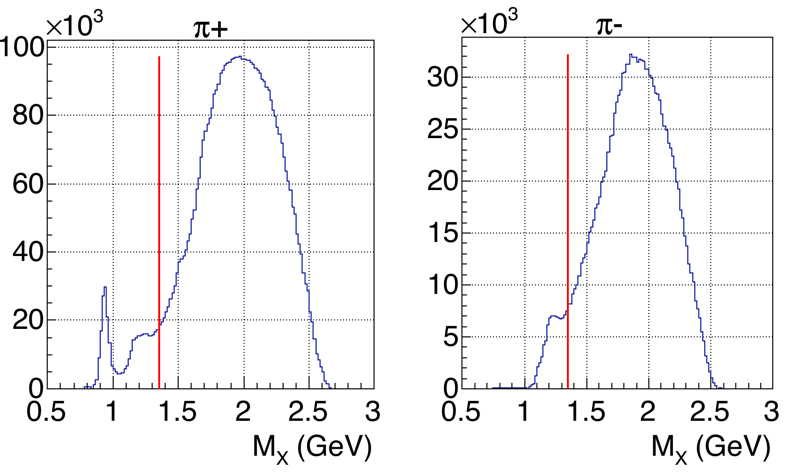
\includegraphics[width=3.0in,height=1.5in]{plots/missingMassCut.png}
\caption{(Color online) The missing mass distribution for $ep \rightarrow e\pi^+ X$ (left) and  $ep \rightarrow e\pi^- X$ (right) events. 
The vertical red line shows the cut of 1.35 GeV. Events to the left of this line are removed from the sample.}
\label{fig:pipMissingMassCut}
\end{figure}
%

A major challenge in extraction of $\phi_h$ distributions is the handling of the detector acceptance, both geometrical acceptance (the location of active detector elements) and the efficiency in the active regions.
This is done using Monte Carlo simulations.
A LUND-MC based event generator (PEPSI~\cite{Mankiewicz:1991dp}) was used to create a realistic large set of events (several iterations were done to make the set ``realistic'') which were passed through a GEANT based simulation of the CLAS detector.
For a given kinematic space, the acceptance is equal to the number of reconstructed events divided by the number of generated events.
The number of events in the E1-f data is then divided by the acceptance to get a corrected value for the number of events.
After events have been selected and binned, and after all corrections, including bin centering corrections,  have been applied, 
a table of values of normalized counts in elementary bins has been extracted in 5-dimensional $x$-$Q^2$-$z$-$\Phperp^2$-$\phi_h$ phase space.

HAPRAD version 2.0 \cite{Akushevich:1999hz,Akushevich:2007jc} was used to calculate radiative corrections for each bin by calculating $\sigma_{rad+tail} \left( x, Q^2, z, P_{h\perp}^2, \phi_h \right)$ for a given \allowbreak $\sigma_{Born} \left( x, Q^2, z, P_{h\perp}^2, \phi_h \right)$ which is obtained from a model.
The radiative correction factor is then simply
\begin{equation}
\begin{split}
\label{eq:RCfactor}
& RC\ factor \left( x, Q^2, z, P_{h\perp}^2, \phi_h \right) =
\\
& \frac{\sigma_{rad+tail} \left( x, Q^2, z, P_{h\perp}^2, \phi_h \right)}{\sigma_{Born} \left( x, Q^2, z, P_{h\perp}^2, \phi_h \right)}
\end{split}
\end{equation}
and the Born cross-section can be obtained by dividing the measured cross-section by the RC factor, i.e., $\sigma_{Born} = \sigma_{measured}/\text{RC factor}$.
Three different models were used to study model dependence of radiative corrections.

Fourteen sources of systematic error were studied.
The systematic error on the final result due to a given source is the RMS of the deviations of the modified result from the original, i.e. the error from source $i$ is
%
\begin{equation}
\label{eq:RMS}
\Delta_{RMS}^i = \frac{\sqrt{\sum_j^{N_v^i} \Delta_j^2}}{\sqrt{N_v^i}}
\end{equation}
%
where $\Delta_j$ is the difference between the final result with the nominal value and the final result with variation $j$, and $N_v^i$ is the number of variations for source $i$.
Main sources of systematic uncertainties include the accetance and variations between the six sectors of CLAS.
%The full list is shown in Table~\ref{Table:accep}


To extract the $\phi_h$-independent term ($A_0$) and azimuthal moments ($A_{UU}^{\cos\phi_h}$ and $A_{UU}^{\cos 2\phi_h}$), the $\phi_h$ distributions for charged pions for each $x-Q^2-z-P_{h\perp}^2$ bin are fit with the function $a(1 + b\cos\phi_h + c\cos 2\phi_h)$.
The parameters $a$, $b$, and $c$ then directly give $A_0$, $A_{UU}^{\cos\phi_h}$, and $A_{UU}^{\cos 2\phi_h}$ for each $x-Q^2-z-P_{h\perp}^2$ bin.
A complete table of results can be found in the ancillary files.
Several representitive plots are shown here in figure~\ref{fig:A0AcAcc_zPT2bins_x1QQ1_final}, which shows $A_0$, $A_{UU}^{\cos\phi_h}$, and $A_{UU}^{\cos 2\phi_h}$ vs $P_{h\perp}^2$ for several $z$ bins for both pion channels.
%
\begin{figure}[htp]
\centering
%\vspace{-1.5cm}
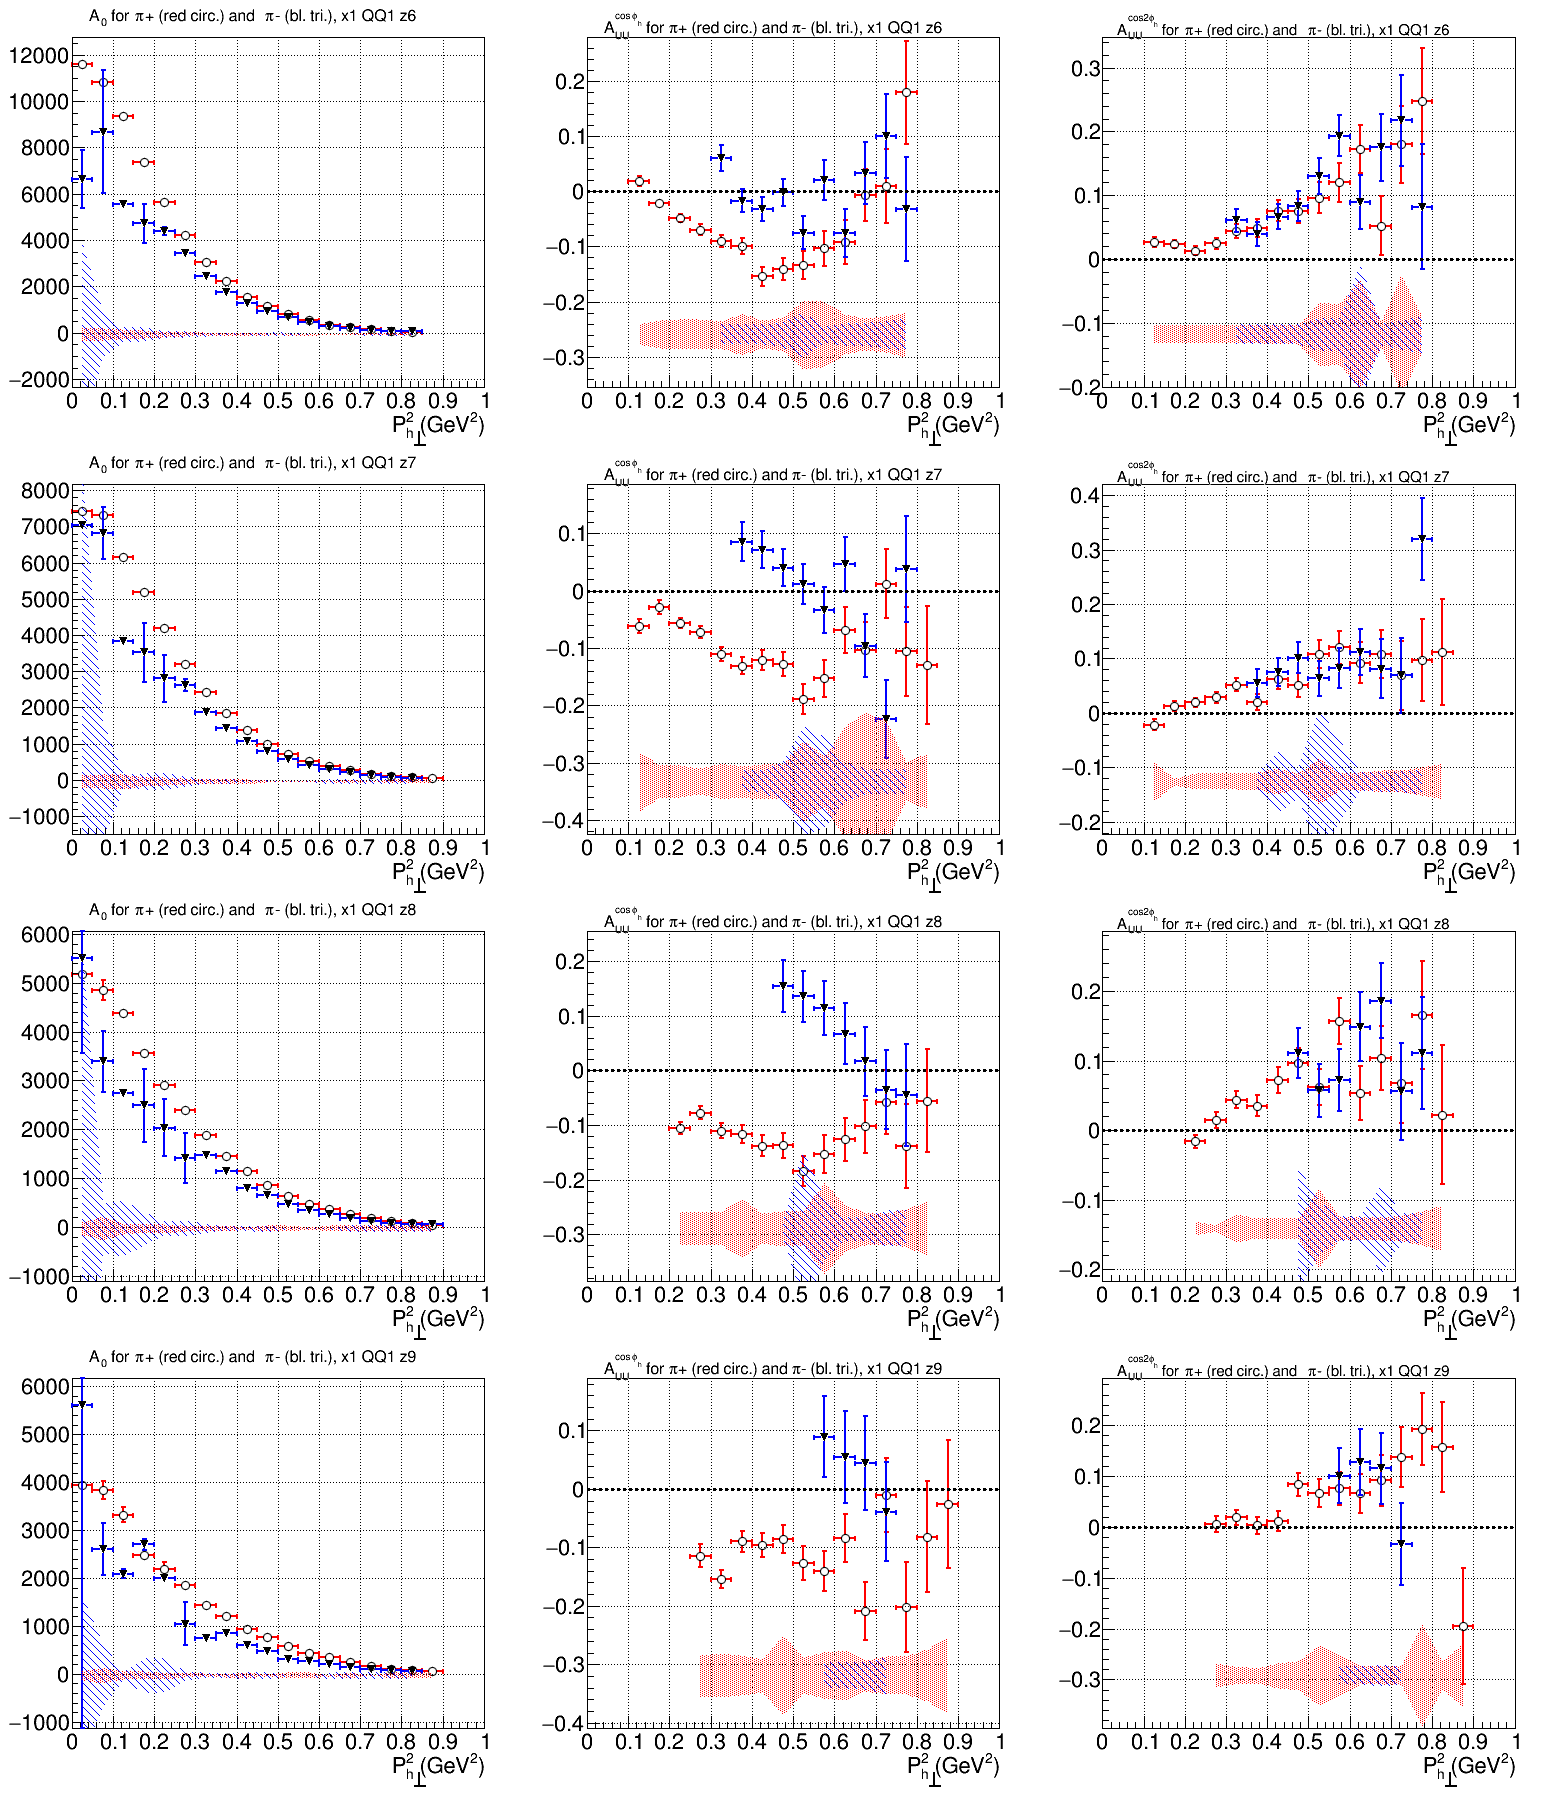
\includegraphics[width=3.5in]{plots/A0AcAcc_zPT2bins_x1QQ1_final.png}
\caption{(Color online) $A_0$ (left column), $A_{UU}^{\cos\phi_h}$ (right column), and $A_{UU}^{\cos 2\phi_h}$ (right column) vs $P_{h\perp}^2$ for both pion channels. The $x$-$Q^2$ bin is fixed (the high $Q^2$ of $0.2 < x < 0.3$). Several $z$ bins are shown: $0.30 < z < 0.35$ (top row), $0.35 < z < 0.40$ (second row), $0.40 < z < 0.45$ (third row), $0.45 < z < 0.50$ (bottom row).}
\label{fig:A0AcAcc_zPT2bins_x1QQ1_final}
\end{figure}

A similar measurement has been published by the CLAS Collaboration using \mbox{E1-6} data~\cite{Osipenko:2008rv}.
However, it only measures the $\pi^+$ channel and has a more limited kinematic range.
A comparison for the $\pi^+$ channel in overlapping kinematic ranges is done here.
In order to have a meaningful comparison, the binning scheme used here was temporarily changed to match that of~\cite{Osipenko:2008rv}.
Figure~\ref{fig:osipenkoComparisonVPT2_2zBins} shows the comparison between E1-f (red up-triangles) and E1-6 (blue down-triangles) as a function of $\Phperp^2$ for two $z$ bins ($0.29 < z < 0.32$ (left column) and $0.32 < z < 0.35$ (right column)) for the $\pi^+$ channel.
The results show clear agreement, both qualitatively and quantitatively, implying good consistency between measurements.
%
\begin{figure}[htp]
\centering
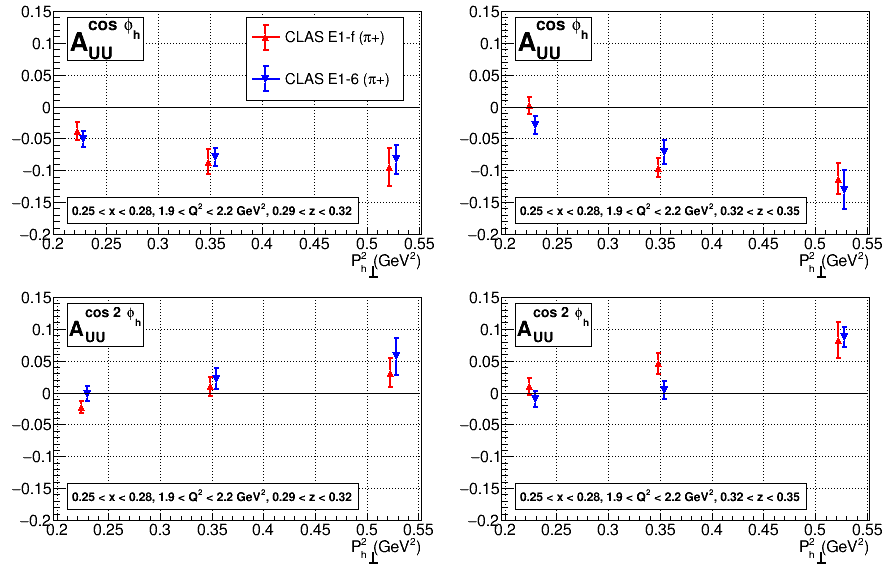
\includegraphics[width=3.5in]{plots/osipenkoComparisonVPT2_2zBins.png}
\caption{(Color online) $A_{UU}^{\cos \phi_h}$ (top row) and $A_{UU}^{\cos 2\phi_h}$ (bottom row) vs $P_{h\perp}^2$ for two $z$ bins ($0.29 < z < 0.32$ (left column) and $0.32 < z < 0.35$ (right column)) for the $\pi^+$ channel for E1-f (red up-triangles) and E1-6 (blue down-triangles). Only the statistical error bars are shown here.}
\label{fig:osipenkoComparisonVPT2_2zBins}
\end{figure}


The measured $cos 2 \phi_h$ moment for $\pi^+$ and $\pi^-$ in most of the kinematics are close to each other indicating the contribution from the Boer-Mulders effect may not be dominant.
The $\rm cos \phi_h$ asymmetry gets contributions only at sub-leading twist and can be used to constrain the related terms~\cite{Cahn:1978se,Anselmino:2005nn,Berger:1979xz}.
The formalism based on the twist-3 approach could be tested in $Q^2$ dependence of $\cos\phi_h$ modulations.  In Fig.~\ref{fig:clas-hermes}, CLAS measurements are compared with corresponding measurements from HERMES experiment~\cite{Airapetian:2012yg}.
After taking into account the kinematic factors in the expression
of the $\cos\phi_h$ modulation and $\phi_h$ independent terms (\cite{Bacchetta:2006tn})
\begin{eqnarray}
f(y)\approx \frac{(2-y)\sqrt{1-y}}{1-y+y^{2}/2} ,
\label{fy}
\end{eqnarray}
the CLAS and HERMES measurements are found to 
be consistent with each other in a wide range of $Q^2$, as shown in Figs.~\ref{fig:clas-hermes}, indicating that at energies as low as 5-6 GeV, the
behavior of azimuthal modulations are similar to higher energy measurements. 
For comparison, the lowest $\xbj$ CLAS bin and highest $\xbj$ HERMES bins were used with equal average value of $\xbj\approx$ 0.19, $z\approx$ 0.45 and $\Phperp^2 \approx$ 0.42 GeV$^2$.

The CLAS data provide significant improvements in the precision of azimuthal moments for the kinematic region where the two data sets overlap, and they extend the measurements to the large $\xbj$ region not accessible at HERMES.

The $cos \phi_h$ modulations for $\pi^+$ and $\pi^-$ differ considerably, sometimes with opposite signs inticating the Boer-Mulders effect in cosine modulations at lower energies plays a more significant role than expected from higher energy measurements.
A possible suppression of the Cahn effect due to phase space limitations, which play a more important role at lower beam energies, has been discussed by Prokudin et al.
\begin{figure}[h]
\begin{center}
%\includegraphics[height=.25\textheight,width=0.4\textwidth]{plots/her-clas-q2-pip-x0.19.z045.pt0.42.pp.pdf}
\includegraphics[height=.25\textheight,width=0.4\textwidth]{plots/hermes_plot_copy.pdf}
\end{center}
\caption{(Color online) The $\cos\phi_h$ modulations in $\pi^\pm$ SIDIS plotted vs $Q^2$. Filled symbols are for $\pi^+$ and open symbols for $\pi^-$.
The triangles CLAS and open symbols are for HERMES~\cite{Airapetian:2012yg}.}
\label{fig:clas-hermes}
\end{figure}


 
%\section{Conclusions}

In summary, we have presented measurements of the kinematic dependences of the azimuthal modulations in semi-inclusive $\pi ^\pm$ electroproduction from the E1-f CLAS data set as a function of $\xbj$, $Q^2$, $z$, and $\Phperp^2$.
%The $\cos \phi_h$ amplitude was extracted as a function of $\xbj$ and transverse pion momentum $\Phperp$, for  $0.4<z<0.7$.
The $\cos \phi_h$ moment shows considerable dependence on the flavor of final state. The results are compared with published HERMES data~\cite{Airapetian:2012yg}, 
providing  a significant improvement in precision and can serve as an important input for studies of higher-twist effects.
The  $Q^2$-dependence of the $\cos\phi_h$ modulation is consistent with 
the twist-3 nature of the contribution and is consistent with measurements performed at much higher energies and $Q^2$.

We thank A. Prokudin and Peter Schweitzer for useful and stimulating discussions.
We would like to acknowledge the outstanding efforts of the staff of the 
Accelerator and the Physics Divisions at JLab that made this experiment possible.
This work was supported in part by 
the National Science Foundation, 
the Italian Istituto Nazionale di Fisica Nucleare, 
the French Centre National de la Recherche Scientifique,
the French Commissariat \`{a} l'Energie Atomique, 
the National Reseach Foundation of Korea,
the UK Science and Technology Facilities Council (STFC),
the EU FP6 (HadronPhysics2, Grant Agreement number 227431),
the Physics Department at Moscow State University
and Chile grant FONDECYT N 1100872.
The Jefferson Science Associates (JSA) operates the Thomas Jefferson National Accelerator Facility for the United States Department of Energy under contract DE-AC05-06OR23177.

\begin{table*}[ht]
  \begin{center}	
    \begin{tabular}{|c|c|c|c|c||c||c||c|c|c|}
       \hline	
	  {$<P_T>$} & {$<z>$} & {$<\xbj >$} & {$<Q^2 >$} & {$<y>$} & A0 & {$A^{\cos\phi_h}_{UU}$} & {$A^{\cos 2\phi_h}_{LU}$} & {$\pm stat.$}  & {$\pm syst.$}\\
	  \hline 
	    \hline 
{0.138 } &  {0.507} & {0.160} & {1.36} & {0.786} & {0.786} & {0.786} & {0.0081} &  {0.0054} & {0.0053}\\
{0.138 } &  {0.507} & {0.160} & {1.36} & {0.786} & {0.786} & {0.786} & {0.0081} &  {0.0054} & {0.0053}\\
	  \hline
    \end{tabular}	
    \caption{The $\phi_h$-independent term ($A_0$) and  moments $A^{\cos \phi_h}_{UU}$ and  $A^{\cos 2\phi_h}_{UU}$ and their statistical and systematic uncertainties at average values of $P_T$, $z$, $\xbj$, $Q^2$ and $y$. An additional 3\% uncertainty from relative uncertainty from radiative effects should be added to the total uncertainty.} 
    \label{aluxbtb}
  \end{center}	
\end{table*}
%\bibliographystyle{model1a-num-names}
%\bibliographystyle{elsevier}

%\bibliographystyle{elsarticle-num}
\bibliography{3dstructure.bib}

\end{document}

%and $\boldsymbol{p_T}$ and $\boldsymbol{k_T}$ are the intrinsic quark transverse momenta in the distribution function (DF) and fragmentation function (FF), respectively.
